\documentclass[compress]{beamer}
\usepackage{ifthen,verbatim}

\newcommand{\isnote}{}
\xdefinecolor{lightyellow}{rgb}{1.,1.,0.25}
\xdefinecolor{darkblue}{rgb}{0.1,0.1,0.7}
\xdefinecolor{darkgreen}{rgb}{0.1,0.7,0.1}

%% Uncomment this to get annotations
%% \def\notes{\addtocounter{page}{-1}
%%            \renewcommand{\isnote}{*}
%% 	   \beamertemplateshadingbackground{lightyellow}{white}
%%            \begin{frame}
%%            \frametitle{Notes for the previous page (page \insertpagenumber)}
%%            \itemize}
%% \def\endnotes{\enditemize
%% 	      \end{frame}
%%               \beamertemplateshadingbackground{white}{white}
%%               \renewcommand{\isnote}{}}

%% Uncomment this to not get annotations
\def\notes{\comment}
\def\endnotes{\endcomment}

\setbeamertemplate{navigation symbols}{}
\setbeamertemplate{headline}{\mbox{ } \hfill
\begin{minipage}{5.5 cm}
\vspace{-0.75 cm} \small
\end{minipage} \hfill
\begin{minipage}{4.5 cm}
\vspace{-0.75 cm} \small
\begin{flushright}
\ifthenelse{\equal{\insertpagenumber}{1}}{}{Jim Pivarski \hspace{0.2 cm} \insertpagenumber\isnote/\pageref{numpages}}
\end{flushright}
\end{minipage}\mbox{\hspace{0.2 cm}}\includegraphics[height=1 cm]{../cmslogo} \hspace{0.1 cm} \includegraphics[height=1 cm]{../tamulogo} \hspace{0.01 cm} \vspace{-1.05 cm}}

\begin{document}
\begin{frame}
\vfill
\begin{center}
\textcolor{darkblue}{\Large DT and CSC Alignments for \\ \vspace{0.25 cm} 2$^{\mbox{\scriptsize nd}}$ CRAFT-09 Reprocessing}

\vfill
\begin{columns}
\column{0.3\linewidth}
\begin{center}
\large
\textcolor{darkblue}{Jim Pivarski}
\end{center}
\end{columns}

\begin{columns}
\column{0.3\linewidth}
\begin{center}
\scriptsize
{\it Texas A\&M University}
\end{center}
\end{columns}

\vfill
30 October, 2009

\end{center}
\end{frame}

%% \begin{notes}
%% \item This is the annotated version of my talk.
%% \item If you want the version that I am presenting, download the one
%% labeled ``slides'' on Indico (or just ignore these yellow pages).
%% \item The annotated version is provided for extra detail and a written
%% record of comments that I intend to make orally.
%% \item Yellow notes refer to the content on the {\it previous} page.
%% \item All other slides are identical for the two versions.
%% \end{notes}

\small

\begin{frame}
\frametitle{Outline}
\begin{itemize}\setlength{\itemsep}{0.5 cm}
\item DT Alignment
\begin{itemize}
\item parameters
\item global adjustment
\item differences with respect to hardware $+$ link
\item segment difference plots
\item distribution of medians
\item map plots
\item fit plots
\end{itemize}

\item CSC Alignment
\begin{itemize}
\item parameters
\item ring adjustments
\item table of ring corrections
\end{itemize}

\item Location of files
\end{itemize}
%% \hspace{-0.83 cm} \textcolor{darkblue}{\Large Outline2}
\end{frame}


\begin{frame}
\frametitle{DT alignment parameters}

\scriptsize
\vspace{-0.25 cm}
\begin{itemize}
\item \scriptsize Sequence:
\begin{enumerate}
\scriptsize \item \scriptsize Barrel\_Opt210-56.db: Hardware $+$ Link-to-AR $+$ internal layer alignment
\item \scriptsize adjust whole barrel global $\delta_x$, $\delta_y$, $\delta_{\phi_z}$ by hand
\item \scriptsize track-based chamber alignment (keeping $\delta_{\phi_x}$ fixed)
\end{enumerate}
\item \scriptsize Where each final aligned position/orientation comes from:
\begin{itemize}
\item \scriptsize all layers/superlayers relative to chamber center: \textcolor{darkblue}{(1)} survey $+$ tracks
\item \scriptsize chambers poorly illuminated by cosmic rays, all parameters:

\textcolor{darkblue}{(1)} Hardware with \textcolor{darkblue}{(2)} global adjustment
\item \scriptsize all chambers local $\delta_{\phi_x}$, station~4 $\delta_y$, $\delta_z$, $\delta_{\phi_y}$: \textcolor{darkblue}{(1)} and \textcolor{darkblue}{(2)}
\item \scriptsize well-illuminated chambers, other params: \textcolor{darkblue}{(3)} \mbox{track-based chamber alignment\hspace{-1 cm}}
\end{itemize}
\item \scriptsize Track-based chamber alignment parameters
\begin{itemize}
\item \scriptsize Dataset: \mbox{\tiny \tt /Cosmics/CRAFT09-StreamMuAlGlobalCosmics-CRAFT09\_R\_V4\_CosmicsSeq\_v1/ALCARECO\hspace{-2 cm}}
\item \scriptsize Run range: 109011--109624 (tracker ``peak mode'')
\item \scriptsize Release: CMSSW\_3\_2\_7
\item \scriptsize GlobalTag: CRAFT09\_R\_V4::All
\item \scriptsize Aligned parameters: stations~1--3 $\delta_x$, $\delta_y$, $\delta_z$, $\delta_{\phi_y}$, $\delta_{\phi_z}$

\textcolor{white}{Aligned parameters:} station~4 $\delta_x$, $\delta_{\phi_y}$, $\delta_{\phi_z}$
\item \scriptsize Tracks: 100 $<$ $p_T$ $<$ 200~GeV, \#tracker hits $\ge$ 15, tracker $\chi^2/\mbox{ndf}$ $<$ 10, no rejection of TID/TEC
\item \scriptsize No special correction for $\vec{B}(\vec{x})$, $dE/dx$
\item \scriptsize Criterion for alignment: at least 30 hits and no Minuit fit failure
\item \scriptsize 5 iterations (2 are necessary for most chambers)
\end{itemize}
\end{itemize}
\end{frame}

\begin{frame}
\frametitle{Global adjustment}

\begin{columns}
\column{0.7\linewidth}
\includegraphics[height=\linewidth, angle=90]{NOV4DT_vs_HARDWARE_phi.pdf}

\includegraphics[height=\linewidth, angle=90]{NOV4DT_vs_HARDWAREadjust_phi.pdf}

\column{0.4\linewidth}
\begin{itemize}
\item Plotting differences between hardware $+$ link geometry and track-based geometry
\item Global adjustment: $\delta_x = 0.6$~mm, $\delta_y = 3.8$~mm, $\delta_{\phi_z} = 0.6$~mrad
\item Almost perfect in $\delta_x$
\item $\delta_y$ and $\delta_{\phi_z}$ are:
\end{itemize}

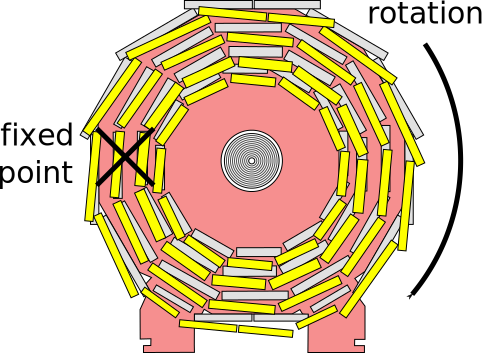
\includegraphics[width=0.9\linewidth]{adjustment_cartoon.pdf}
\end{columns}
\end{frame}

\begin{frame}
\frametitle{Compared to photogrammetry\ldots}

\begin{columns}
\column{0.7\linewidth}
\mbox{\hspace{0.5 cm}\includegraphics[height=\linewidth, angle=90]{final_vs_PG09_phi.pdf}}

\mbox{\hspace{0.5 cm}\includegraphics[height=\linewidth, angle=90]{final_vs_PG09barrelplus_phi.pdf}}

\column{0.45\linewidth}
\begin{itemize}
\item Plotting differences between PG $+$ cavern survey and track-based geometry
\item Global adjustment: $\delta_x = 2.2$~mm, $\delta_y = 5.1$~mm, $\delta_{\phi_z} = 0.6$~mrad
\item Not apples-to-apples:
\begin{itemize}
\item \mbox{cavern global coords,\hspace{-1 cm}} \\ not tracker coords
\item different internal \mbox{geometry? (Luca?)\hspace{-2 cm}}
\item $\dfrac{1}{10}$ track sample
\end{itemize}
\item But PG vs.\ tracks is narrower than HW vs.\ tracks
\end{itemize}
\end{columns}
\end{frame}

\begin{frame}
\frametitle{Hardware vs.\ track-based}

\begin{columns}
\column{0.5\linewidth}
\includegraphics[height=\linewidth, angle=90]{NOV4DT_vs_HARDWAREadjust_x.pdf}

\includegraphics[height=\linewidth, angle=90]{NOV4DT_vs_HARDWAREadjust_y.pdf}

\includegraphics[height=\linewidth, angle=90]{NOV4DT_vs_HARDWAREadjust_z.pdf}

\column{0.5\linewidth}
\begin{itemize}
\item Plotting differences between globally-adjusted hardware and track-based geometry
\item Local $x'$, $y'$, and $z'$ vs.\ $\phi$ \mbox{(prime indicates consistent sign)\hspace{-1 cm}}
\begin{itemize}
\item $x'$: anti-clockwise $r\phi$
\item $y'$: parallel to beamline, pointing west
\item $z'$: radial, pointing inward
\end{itemize}
\item Semi-regular patterns emerge from the differences: could indicate discrepancies in chamber center assumptions
\begin{itemize}
\item especially sectors 8, 9, 10 ($-2.8 < \phi < -1.4$)
\end{itemize}
\end{itemize}
\end{columns}
\end{frame}

\begin{frame}
\frametitle{Segment differences (1)}

\begin{itemize}
\item Standard segment-extrapolation test was unavailable this week, so I implemented a version with more realistic track-propagation
\end{itemize}

\vspace{-0.4 cm}
\begin{columns}
\column{0.45\linewidth}
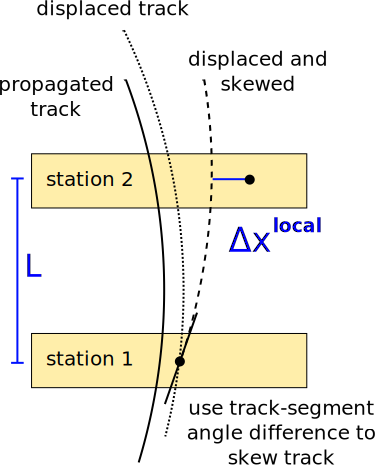
\includegraphics[width=\linewidth]{segdiff_cartoon.pdf}

\column{0.55\linewidth}
\begin{itemize}
\item Local angle difference is difference of residuals with respect to the propagated tracker track

$\Delta \frac{dx}{dz}^{\mbox{\scriptsize local}} = \Delta \frac{dx}{dz}_{\mbox{\scriptsize st.2}} - \Delta \frac{dx}{dz}_{\mbox{\scriptsize st.1}}$

\item Local position difference also needs to correct for segment direction by a linear transformation (see left)

\mbox{\hspace{-0.75 cm}$\Delta x^{\mbox{\scriptsize local}} = \Delta x_{\mbox{\scriptsize st.2}} - \Delta x_{\mbox{\scriptsize st.1}} - L \cdot \Delta \frac{dx}{dz}_{\mbox{\scriptsize st.1}}$}

\item In the limit of linear track propagation, this is exactly a linear segment extrapolation

\item This is how Millepede applies track corrections to realistically-modelled tracks (small linear transforms)

\end{itemize}
\end{columns}
\end{frame}

\begin{frame}
\frametitle{Segment differences (2)}

\begin{columns}
\column{0.7\linewidth}
\includegraphics[width=\linewidth]{NOV4_segdiffs/dt13_resid_C_05_12.png}

\includegraphics[height=\linewidth, angle=90]{NOV4_segdiff_x_whze.pdf}
\column{0.4\linewidth}
\begin{itemize}
\item Two fits: linear $q/p_T \to 0$ and Gaussian of positive and
  negative separately
\begin{itemize}
\item linear $q/p_T \to 0$ results are {\it filled} \textcolor{blue}{circles,} \textcolor{red}{squares,} and \textcolor{darkgreen}{triangles}
\item \mbox{average of Gaussian\hspace{-1 cm}} \\ fits are {\it hollow}
\end{itemize}

\item 1.7--2.5$\times$ higher resolution in raw distributions and
  final results: RMS of stations 1--3 is 0.3~mm rather than 0.7~mm

\item Reveals non-zero biases in \mbox{alignment: $\mathcal{O}(\mbox{0.2~mm})$\hspace{-1 cm}}

\end{itemize}
\end{columns}
\end{frame}

\begin{frame}
\frametitle{Segment differences: wheel $-$2}

{\scriptsize
\begin{itemize}
\item A complete set of linear and Gaussian fits is in SegmentDifferences.pdf
\item Careful of difference in vertical scales
\end{itemize}}

\begin{center} Globally-adjusted hardware geometry \end{center}

\vspace{-0.1 cm}
\includegraphics[height=0.5\linewidth, angle=90]{NOV4_segdiff_HW_x_whm2.pdf}
\includegraphics[height=0.5\linewidth, angle=90]{NOV4_segdiff_HW_dxdz_whm2.pdf}

\begin{center} Track-based geometry \end{center}

\vspace{-0.1 cm}
\includegraphics[height=0.5\linewidth, angle=90]{NOV4_segdiff_x_whm2.pdf}
\includegraphics[height=0.5\linewidth, angle=90]{NOV4_segdiff_dxdz_whm2.pdf}
\end{frame}

\begin{frame}
\frametitle{Segment differences: wheel $-$1}

{\scriptsize
\begin{itemize}
\item A complete set of linear and Gaussian fits is in SegmentDifferences.pdf
\item Careful of difference in vertical scales
\end{itemize}}

\begin{center} Globally-adjusted hardware geometry \end{center}

\vspace{-0.1 cm}
\includegraphics[height=0.5\linewidth, angle=90]{NOV4_segdiff_HW_x_whm1.pdf}
\includegraphics[height=0.5\linewidth, angle=90]{NOV4_segdiff_HW_dxdz_whm1.pdf}

\begin{center} Track-based geometry \end{center}

\vspace{-0.1 cm}
\includegraphics[height=0.5\linewidth, angle=90]{NOV4_segdiff_x_whm1.pdf}
\includegraphics[height=0.5\linewidth, angle=90]{NOV4_segdiff_dxdz_whm1.pdf}
\end{frame}

\begin{frame}
\frametitle{Segment differences: wheel 0}

{\scriptsize
\begin{itemize}
\item A complete set of linear and Gaussian fits is in SegmentDifferences.pdf
\item Careful of difference in vertical scales
\end{itemize}}

\begin{center} Globally-adjusted hardware geometry \end{center}

\vspace{-0.1 cm}
\includegraphics[height=0.5\linewidth, angle=90]{NOV4_segdiff_HW_x_whze.pdf}
\includegraphics[height=0.5\linewidth, angle=90]{NOV4_segdiff_HW_dxdz_whze.pdf}

\begin{center} Track-based geometry \end{center}

\vspace{-0.1 cm}
\includegraphics[height=0.5\linewidth, angle=90]{NOV4_segdiff_x_whze.pdf}
\includegraphics[height=0.5\linewidth, angle=90]{NOV4_segdiff_dxdz_whze.pdf}
\end{frame}

\begin{frame}
\frametitle{Segment differences: wheel $+$1}

{\scriptsize
\begin{itemize}
\item A complete set of linear and Gaussian fits is in SegmentDifferences.pdf
\item Careful of difference in vertical scales
\end{itemize}}

\begin{center} Globally-adjusted hardware geometry \end{center}

\vspace{-0.1 cm}
\includegraphics[height=0.5\linewidth, angle=90]{NOV4_segdiff_HW_x_whp1.pdf}
\includegraphics[height=0.5\linewidth, angle=90]{NOV4_segdiff_HW_dxdz_whp1.pdf}

\begin{center} Track-based geometry \end{center}

\vspace{-0.1 cm}
\includegraphics[height=0.5\linewidth, angle=90]{NOV4_segdiff_x_whp1.pdf}
\includegraphics[height=0.5\linewidth, angle=90]{NOV4_segdiff_dxdz_whp1.pdf}
\end{frame}

\begin{frame}
\frametitle{Segment differences: wheel $+$2}

{\scriptsize
\begin{itemize}
\item A complete set of linear and Gaussian fits is in SegmentDifferences.pdf
\item Careful of difference in vertical scales
\end{itemize}}

\begin{center} Globally-adjusted hardware geometry \end{center}

\vspace{-0.1 cm}
\includegraphics[height=0.5\linewidth, angle=90]{NOV4_segdiff_HW_x_whp2.pdf}
\includegraphics[height=0.5\linewidth, angle=90]{NOV4_segdiff_HW_dxdz_whp2.pdf}

\begin{center} Track-based geometry \end{center}

\vspace{-0.1 cm}
\includegraphics[height=0.5\linewidth, angle=90]{NOV4_segdiff_x_whp2.pdf}
\includegraphics[height=0.5\linewidth, angle=90]{NOV4_segdiff_dxdz_whp2.pdf}
\end{frame}

\begin{frame}
\frametitle{Distribution of medians (1)}
\begin{itemize}
\item Each histogram entry is one chamber's median of residuals
\begin{itemize}
\item tests self-consistency; median is a different way to be insensitive to residuals tails than the fitting method
\end{itemize}
\item CRAFT-08 RMS $\Delta x$: 0.190~mm $\Delta \frac{dx}{dz}$: 0.085~mrad $\Delta y$: 0.166~mm $\Delta \frac{dy}{dz}$: 0.885~mrad; now we don't align $\Delta \frac{dy}{dz}$, which feeds into $\Delta y$
\end{itemize}

\includegraphics[height=\linewidth, angle=90]{NOV4DT_median_all.pdf}
\end{frame}

\begin{frame}
\frametitle{Distribution of medians (2)}
\begin{itemize}
\item CRAFT-08 RMS $\Delta x$: 0.190~mm $\Delta \frac{dx}{dz}$: 0.085~mrad $\Delta y$: 0.166~mm $\Delta \frac{dy}{dz}$: 0.885~mrad; now we don't align $\Delta \frac{dy}{dz}$, which feeds into $\Delta y$
\item Now also restricting to the set of CRAFT-08 chambers \\ (wheel $-$1, 0, $+$1, all sectors except 1 and 7)
\end{itemize}

\includegraphics[height=\linewidth, angle=90]{NOV4DT_median_goodDT.pdf}
\end{frame}

\begin{frame}
\frametitle{Map plots}

\begin{columns}
\column{0.7\linewidth}
\includegraphics[width=\linewidth]{NOV4_mapplots_HW/DTvsphi_st1whC_x.png}

\includegraphics[width=\linewidth]{NOV4_mapplots/DTvsphi_st1whC_x.png}

\column{0.4\linewidth}
\begin{itemize}
\item Residuals as a function of $\phi$, $z$ with chamber boundaries as dashed lines, color scale is 2-D plot, points are profile
\item Top: globally-adjusted hardware geometry, bottom: track-based
\item If the discrepancy were due to distortions in the track source or propagation, it wouldn't change abruptly at chamber boundaries
\item Complete set in MapPlots.pdf
\end{itemize}
\end{columns}
\end{frame}

\begin{frame}
\frametitle{Fit plots}
\begin{columns}
\column{0.7\linewidth}
\includegraphics[width=\linewidth]{NOV4_fitfunctions/MBwhCst1sec10_bellcurves.png}

\includegraphics[width=\linewidth]{NOV4_fitfunctions/MBwhCst1sec10_polynomials.png}

\column{0.4\linewidth}
\begin{itemize}
\item Overlay of fit function on residuals projections \mbox{(after alignment)}
\item Bell-curves are Gaussians $+$ tails, should be centered (except unaligned $\Delta \frac{dy}{dz}$)
\item Scatter plots are position-angle correlations, should {\it not} be flat (propagation)
\item Points with error bars are residuals versus everything, should be flat (geometric)
\item Complete set in FitFunctions.pdf
\end{itemize}
\end{columns}
\end{frame}

\begin{frame}
\frametitle{Sawtooth effect?}

\begin{itemize}
\item Sawtooth effect is not very evident, scanning through \mbox{map and fit plots\hspace{-1 cm}}

\item Below is an old example plot showing the sawtooth:

\mbox{\hspace{-1.5 cm}\includegraphics[height=0.7\linewidth, angle=90]{alignmentplots_example2.pdf}}

\vspace{-3.2 cm}
\hfill \includegraphics[width=0.45\linewidth]{NOV4_sawtooth.pdf}

\vspace{-2 cm}
\item $\sim$5~mm difference in $\Delta x$ residuals \\ from $x=-100$ to $+100$~cm

\item How much is it now?  \\ Fit all $\Delta x$ vs.\ $x$ distributions, \\ evaluate at $\pm 100$~cm (new histogram on right)

\item Less than half as large, and not all in the same direction

\item Maybe due to calibration, and that was improved?  (a guess)
\end{itemize}
\end{frame}

\begin{frame}
\frametitle{Relation to tracker}

\scriptsize
\begin{itemize}
\item \scriptsize At the time that all of these plots were made, the tracker
  alignment group was making a final decision between their
  {\tiny \tt HIPCenteredObject.db} and \mbox{\tiny \tt MergedCenteredObject.db\hspace{-1 cm}}
\item \scriptsize Two muon alignments were produced, one for each tracker description in parallel
\item \scriptsize All of the plots shown here were made with
  {\tiny \tt MergedCenteredObject.db}, but the final tracker alignment is
  {\tiny \tt HIPCenteredObject.db}.
\item \scriptsize The differences in muon alignment (DT and CSC) are on the 250~$\mu$m level
\end{itemize}

\includegraphics[width=\linewidth]{trackerdiff_DT.pdf}
\end{frame}

\begin{frame}
\frametitle{CSC alignment parameters}

\scriptsize
\begin{itemize}
\item \scriptsize Sequence:
\begin{enumerate}
\scriptsize \item \scriptsize 2009 hardware alignment ($\delta_z$ and $\delta_{\phi_x}$)
\item \scriptsize adjust each ring's global $\delta_x$, $\delta_y$, $\delta_{\phi_z}$ by hand
\end{enumerate}
\item \scriptsize Where each final aligned position/orientation comes from:
\begin{itemize}
\item \scriptsize all internal layers relative to chamber center: ideal
\item \scriptsize all chambers $\delta_{\phi_x}$ and $\delta_z$: \textcolor{darkblue}{(1)} hardware
\item \scriptsize all chambers $\delta_x$, $\delta_y$, $\delta_{\phi_z}$: \textcolor{darkblue}{(2)} ring adjustment
\end{itemize}
\item \scriptsize Track-based alignment parameters
\begin{itemize}
\item \scriptsize Dataset: \mbox{\tiny \tt /Cosmics/CRAFT09-CSCSkim\_BFieldStudies-CRAFT09\_R\_V4\_CosmicsSeq\_v1/RAW-RECO\hspace{-2 cm}}
\item \scriptsize Run range: 109011--109624 (tracker ``peak mode'')
\item \scriptsize Release: CMSSW\_3\_2\_7
\item \scriptsize GlobalTag: CRAFT09\_R\_V4::All
\item \scriptsize Tracks: 100 $<$ $p_T$ $<$ 200~GeV, \#tracker hits $\ge$ 15, tracker $\chi^2/\mbox{ndf}$ $<$ 10, no rejection of TID/TEC
\item \scriptsize No special correction for $\vec{B}(\vec{x})$, $dE/dx$
\item \scriptsize Alignment performed by fitting map plots
\end{itemize}
\end{itemize}

\vfill
\begin{itemize}
\item \scriptsize Note: statistical errors in individual-chamber alignments are unacceptably high: 1~mrad in $\phi_y$; that's why they were only collectively aligned
\item \scriptsize This procedure compliments the beam-halo procedure well (which aligns individual chambers, but not the rings relative to the tracker)
\end{itemize}
\end{frame}

\begin{frame}
\frametitle{Ring fits (1/8)}
\mbox{\hspace{-0.8 cm}\begin{minipage}{1.15\linewidth}
\includegraphics[height=0.5\linewidth, angle=90]{NOV4_ringfits_before/mem11.pdf}
\includegraphics[height=0.5\linewidth, angle=90]{NOV4_ringfits_before/mep11.pdf}

\vspace{0.25 cm}
\includegraphics[height=0.5\linewidth, angle=90]{NOV4_ringfits_after/mem11.pdf}
\includegraphics[height=0.5\linewidth, angle=90]{NOV4_ringfits_after/mep11.pdf}
\end{minipage}}
\end{frame}

\begin{frame}
\frametitle{Ring fits (2/8)}
\mbox{\hspace{-0.8 cm}\begin{minipage}{1.15\linewidth}
\includegraphics[height=0.5\linewidth, angle=90]{NOV4_ringfits_before/mem12.pdf}
\includegraphics[height=0.5\linewidth, angle=90]{NOV4_ringfits_before/mep12.pdf}

\vspace{0.25 cm}
\includegraphics[height=0.5\linewidth, angle=90]{NOV4_ringfits_after/mem12.pdf}
\includegraphics[height=0.5\linewidth, angle=90]{NOV4_ringfits_after/mep12.pdf}
\end{minipage}}
\end{frame}

\begin{frame}
\frametitle{Ring fits (3/8)}
\mbox{\hspace{-0.8 cm}\begin{minipage}{1.15\linewidth}
\includegraphics[height=0.5\linewidth, angle=90]{NOV4_ringfits_before/mem13.pdf}
\includegraphics[height=0.5\linewidth, angle=90]{NOV4_ringfits_before/mep13.pdf}

\vspace{0.25 cm}
\includegraphics[height=0.5\linewidth, angle=90]{NOV4_ringfits_after/mem13.pdf}
\includegraphics[height=0.5\linewidth, angle=90]{NOV4_ringfits_after/mep13.pdf}
\end{minipage}}
\end{frame}

\begin{frame}
\frametitle{Ring fits (4/8)}
\mbox{\hspace{-0.8 cm}\begin{minipage}{1.15\linewidth}
\includegraphics[height=0.5\linewidth, angle=90]{NOV4_ringfits_before/mem21.pdf}
\includegraphics[height=0.5\linewidth, angle=90]{NOV4_ringfits_before/mep21.pdf}

\vspace{0.25 cm}
\includegraphics[height=0.5\linewidth, angle=90]{NOV4_ringfits_after/mem21.pdf}
\includegraphics[height=0.5\linewidth, angle=90]{NOV4_ringfits_after/mep21.pdf}
\end{minipage}}
\end{frame}

\begin{frame}
\frametitle{Ring fits (5/8)}
\mbox{\hspace{-0.8 cm}\begin{minipage}{1.15\linewidth}
\includegraphics[height=0.5\linewidth, angle=90]{NOV4_ringfits_before/mem22.pdf}
\includegraphics[height=0.5\linewidth, angle=90]{NOV4_ringfits_before/mep22.pdf}

\vspace{0.25 cm}
\includegraphics[height=0.5\linewidth, angle=90]{NOV4_ringfits_after/mem22.pdf}
\includegraphics[height=0.5\linewidth, angle=90]{NOV4_ringfits_after/mep22.pdf}
\end{minipage}}
\end{frame}

\begin{frame}
\frametitle{Ring fits (6/8)}
\mbox{\hspace{-0.8 cm}\begin{minipage}{1.15\linewidth}
\includegraphics[height=0.5\linewidth, angle=90]{NOV4_ringfits_before/mem31.pdf}
\includegraphics[height=0.5\linewidth, angle=90]{NOV4_ringfits_before/mep31.pdf}

\vspace{0.25 cm}
\includegraphics[height=0.5\linewidth, angle=90]{NOV4_ringfits_after/mem31.pdf}
\includegraphics[height=0.5\linewidth, angle=90]{NOV4_ringfits_after/mep31.pdf}
\end{minipage}}
\end{frame}

\begin{frame}
\frametitle{Ring fits (7/8)}
\mbox{\hspace{-0.8 cm}\begin{minipage}{1.15\linewidth}
\includegraphics[height=0.5\linewidth, angle=90]{NOV4_ringfits_before/mem32.pdf}
\includegraphics[height=0.5\linewidth, angle=90]{NOV4_ringfits_before/mep32.pdf}

\vspace{0.25 cm}
\includegraphics[height=0.5\linewidth, angle=90]{NOV4_ringfits_after/mem32.pdf}
\includegraphics[height=0.5\linewidth, angle=90]{NOV4_ringfits_after/mep32.pdf}
\end{minipage}}
\end{frame}

\begin{frame}
\frametitle{Ring fits (8/8)}
\mbox{\hspace{-0.8 cm}\begin{minipage}{1.15\linewidth}
\includegraphics[height=0.5\linewidth, angle=90]{NOV4_ringfits_before/mem41.pdf}
\includegraphics[height=0.5\linewidth, angle=90]{NOV4_ringfits_before/mep41.pdf}

\vspace{0.25 cm}
\includegraphics[height=0.5\linewidth, angle=90]{NOV4_ringfits_after/mem41.pdf}
\includegraphics[height=0.5\linewidth, angle=90]{NOV4_ringfits_after/mep41.pdf}
\end{minipage}}
\end{frame}

\begin{frame}
\frametitle{Table of ring corrections}
\begin{itemize}
\item Grouped items are physically connected to the same disk; values are correlated but not exactly equal within fitting errors
\item Large $\chi^2/\mbox{ndf}$ expected from incomplete chamber alignment
\end{itemize}

\scriptsize
\renewcommand{\arraystretch}{1.1}
\begin{tabular}{c | c c c c}
ring & $\delta_x$ (mm) & $\delta_y$ (mm) & $\delta_{\phi_z}$ (mrad) & $\chi^2/\mbox{ndf}$ \\\hline
ME$-$4/1 & $ 3.20$ $\pm$ $ 0.17$ & $-3.85$ $\pm$ $ 0.29$ & $ 1.78$ $\pm$ $ 0.05$ & 12.7426 \\\hline
ME$-$3/2 & $ 2.03$ $\pm$ $ 0.05$ & $-1.86$ $\pm$ $ 0.08$ & $ 1.95$ $\pm$ $ 0.01$ & 52.4465 \\
ME$-$3/1 & $ 2.77$ $\pm$ $ 0.13$ & $-4.75$ $\pm$ $ 0.21$ & $ 2.61$ $\pm$ $ 0.04$ & 24.2564 \\
ME$-$2/2 & $ 1.87$ $\pm$ $ 0.05$ & $-0.82$ $\pm$ $ 0.07$ & $ 1.55$ $\pm$ $ 0.01$ & 41.8597 \\
ME$-$2/1 & $ 2.54$ $\pm$ $ 0.10$ & $-3.12$ $\pm$ $ 0.17$ & $ 2.37$ $\pm$ $ 0.04$ & 27.4691 \\\hline
ME$-$1/3 & $ 1.93$ $\pm$ $ 0.08$ & $ 1.01$ $\pm$ $ 0.12$ & $ 0.41$ $\pm$ $ 0.01$ & 45.7221 \\
ME$-$1/2 & $ 3.86$ $\pm$ $ 0.06$ & $-2.00$ $\pm$ $ 0.09$ & $ 0.83$ $\pm$ $ 0.01$ & 17.4924 \\
ME$-$1/1 & $ 2.97$ $\pm$ $ 0.11$ & $-4.13$ $\pm$ $ 0.17$ & $ 0.64$ $\pm$ $ 0.05$ & 9.08853 \\\hline
ME$+$1/1 & $ 5.06$ $\pm$ $ 0.11$ & $-0.86$ $\pm$ $ 0.16$ & $ 0.19$ $\pm$ $ 0.05$ & 3.48464 \\
ME$+$1/2 & $ 5.20$ $\pm$ $ 0.06$ & $ 0.92$ $\pm$ $ 0.09$ & $ 0.22$ $\pm$ $ 0.01$ & 17.3722 \\
ME$+$1/3 & $ 4.66$ $\pm$ $ 0.07$ & $ 2.37$ $\pm$ $ 0.11$ & $ 0.05$ $\pm$ $ 0.01$ & 32.8144 \\\hline
ME$+$2/1 & $ 4.94$ $\pm$ $ 0.10$ & $ 3.10$ $\pm$ $ 0.16$ & $ 0.03$ $\pm$ $ 0.04$ & 20.9203 \\
ME$+$2/2 & $ 4.65$ $\pm$ $ 0.04$ & $ 3.41$ $\pm$ $ 0.07$ & $-0.05$ $\pm$ $ 0.01$ & 43.0836 \\
ME$+$3/1 & $ 4.42$ $\pm$ $ 0.14$ & $ 5.72$ $\pm$ $ 0.24$ & $-0.32$ $\pm$ $ 0.05$ & 55.0455 \\
ME$+$3/2 & $ 4.86$ $\pm$ $ 0.05$ & $ 2.98$ $\pm$ $ 0.08$ & $-0.27$ $\pm$ $ 0.01$ & 46.2096 \\\hline
ME$+$4/1 & $\sim 5.13$ $\pm$ $ 0.25$ & $\sim 8.27$ $\pm$ $ 0.30$ & $\sim 0.55$ $\pm$ $ 0.08$ & 78.0725
\end{tabular}
\end{frame}

%% \section*{First section}
%% \begin{frame}
%% \begin{center}
%% \Huge \textcolor{blue}{First section}
%% \end{center}
%% \end{frame}

\begin{frame}
\frametitle{Conclusions}
\begin{itemize}
\item DT alignment constructed from hardware, link, and tracks:

\mbox{\hspace{-1.25 cm} \tiny \tt /afs/cern.ch/user/p/pivarski/public/DTAlignmentRcd\_CRAFT09\_segments-hardware-globalMuons\_3XY\_v8\_offline.db}
\mbox{\hspace{-1.25 cm} \tiny \tt \ldots/DTAlignmentRcd\_CRAFT09\_segments-hardware-globalMuons\_3XY\_v8\_offline\_RELTOIDEAL.xml}
\mbox{\hspace{-1.25 cm} \tiny \tt \ldots/DTAlignmentRcd\_CRAFT09\_segments-hardware-globalMuons\_3XY\_v8\_offline\_RELTONONE.xml}

\begin{itemize}
\item tags: DTAlignmentRcd and DTAlignmentErrorRcd (infinite for unaligned chambers)
\end{itemize}

\item CSC alignment constructed from hardware and tracks:

\mbox{\hspace{-1.25 cm} \tiny \tt /afs/cern.ch/user/p/pivarski/public/CSCAlignmentRcd\_CRAFT09\_hardware-globalMuons\_3XY\_v4\_offline.db}
\mbox{\hspace{-1.25 cm} \tiny \tt \ldots/CSCAlignmentRcd\_CRAFT09\_hardware-globalMuons\_3XY\_v4\_offline\_RELTOIDEAL.xml}
\mbox{\hspace{-1.25 cm} \tiny \tt \ldots/CSCAlignmentRcd\_CRAFT09\_hardware-globalMuons\_3XY\_v4\_offline\_RELTONONE.xml}

\begin{itemize}
\item tags: only CSCAlignmentRcd, use ideal errors
\end{itemize}

\item Corresponding tracker geometry: {\tiny \tt HIPCenteredObject.db}

\begin{itemize}
\item updated Oct 30, 20:15 European time
\end{itemize}

\end{itemize}
\label{numpages}
\end{frame}

\end{document}
